\subsection{Overview of the User Interface}
According to Software Requirement Specification document(SRS), this embedded software system shall provide the graphic user interface for user to interact with the EV3 robot via graphic icons, file input and output. The below is the list of functionalities of GUI mentioned in SRS:
\begin{itemize}
	\item The user is able to control the robot manually.
	\item The user is able to command the robot to move to specific point in the map under manual mode.
	\item The user is able to switch the current mode (Navigation and Manual modes) of the robot.
	\item The user is able to see the obstacles, line track displaced on the map.
	\item The user is able to trace the robot's current position.
	\item The user is able to see the detailed system log including software and hardware of the robot.
	\item The user is able to import and export XML file to define and retrieve the map information.
\end{itemize}

\subsection{Detailed Design of the User Interface}
The GUI is divided into four main parts and listed in Table \ref{GUI Features}. Each part of GUI consists of multiple panels.

\begin{table}[]
	\centering
	\caption{GUI Features}
	\label{GUI Features}
	\begin{tabular}{|p{3cm}|p{2cm}|p{6cm}|}
		\hline
		Name & Component & Related Features \\ \hline
		Manual Control &  & UR13, UR14, FR008, FR009, FR010 \\ \hline
		Map panel  &  & UR03, UR04, UR07, UR12, UR15, FR006, FR012 \\ \hline
		System status and log panels &  & FR015, EM001 \\ \hline
		Other functionalities &  &  UR05, UR06, FR001, FR002, FR003, FR004 \\ \hline
	\end{tabular}
\end{table}

\subsubsection{GUI's screen image}
Fig.5 shows the screen image of GUI for end user perspective. The GUI supports mouse and keyboard devices. Each device is linked to GUI via action listeners established by GUI. When the GUI is created, there are multiply listeners created to listen the events from input devices. The detail actions will be discussed in section 6.2.2  

\begin{figure}[H]
	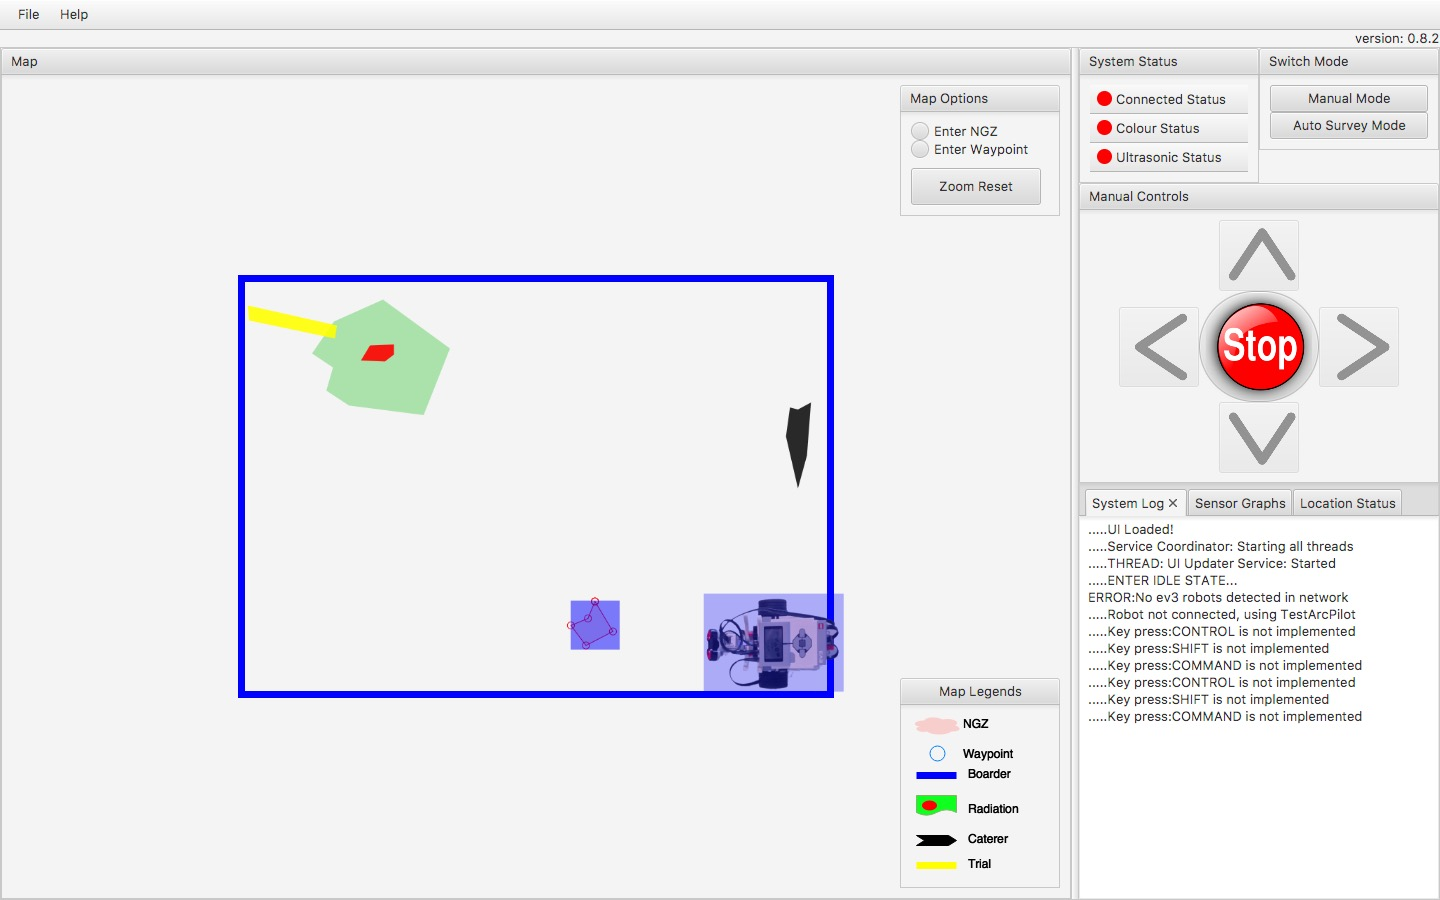
\includegraphics[width=\linewidth]{GUI.png}  % created using www.draw.io
	\caption{Graphic User Interface}
	\label{fig:Graphic User Interface}              
\end{figure}

\subsubsection{Manual Control}
\textbf{Supporting input devices: Keyboard and Mouse}
Manual Control has two listeners for listen the event and determine the actions. One listener is for the event coming from mouse device. The another is for the event coming from keyboard. Fig.6 is the manual control panel \\
\\
\textbf{Listener for listening mouse and keyboard event}\\
The user can use their mouse to click the graphic icons showing on the Manual Control panel to control the robot. Also, the user can use keyboard to fire the event to GUI to control the robot instead. Each button and keyboard listeners have different method to control the robot. For example, if the user click the stop button, the method called onClickStop() will be called and stop the robot movement. The list of methods called by listeners is shown on Table \ref{Method called for Manual Control}.

\begin{figure}[H]
	\centering
	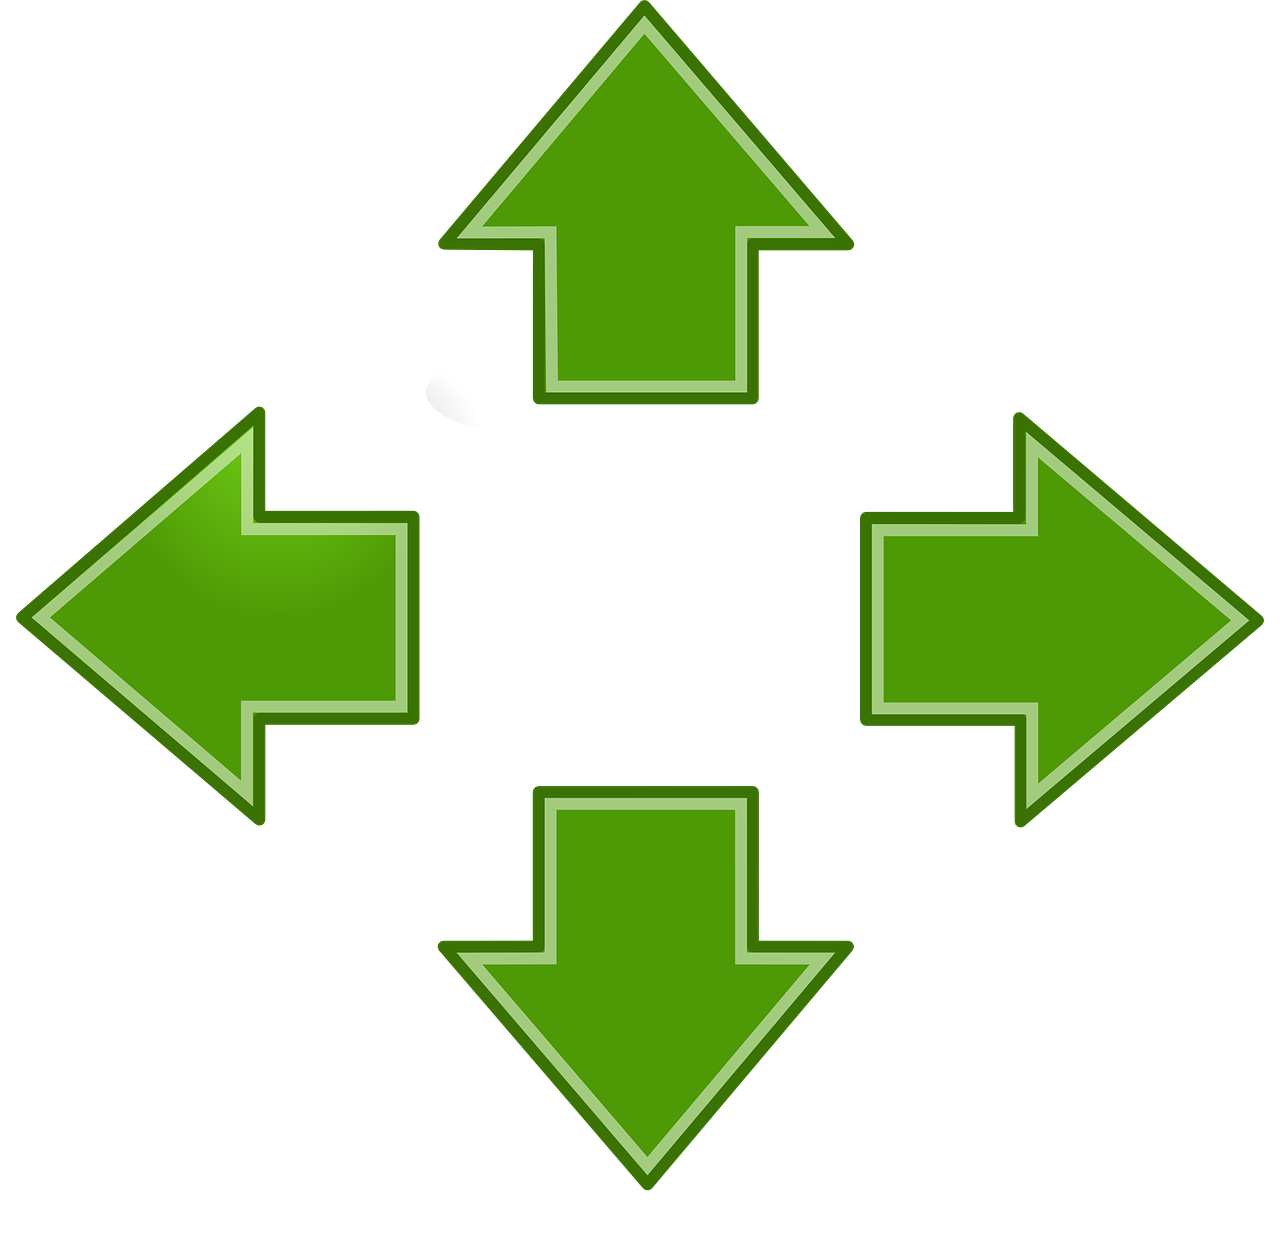
\includegraphics[width=80mm]{Control.png}  % created using www.draw.io
	\caption{Manual control}
	\label{fig:Manual controller}              
\end{figure}

\begin{table}[]
	\centering
	\caption{Method called for Manual Control}
	\label{Method called for Manual Control}
	\begin{tabular}{|l|c|l|l|}
		\hline
		\textbf{Method Name}            & \textbf{Graphic Buttons} & \textbf{KeyBoard Keys} & \textbf{Action} \\ \hline
		\textbf{onClickForward}  & \parbox[c]{1em}{
\includegraphics[width=15mm]{Up.PNG}} & W & Moving Forward  \\ \hline
		\textbf{onClickBackward} & \parbox[c]{1em}{
\includegraphics[width=15mm]{Down.PNG}} & S & Moving Backward \\ \hline
		\textbf{onClickLeft}     & \parbox[c]{1em}{
\includegraphics[width=15mm]{Left.PNG}} & A & Turn Left       \\ \hline
		\textbf{onClickRight}    & \parbox[c]{1em}{
\includegraphics[width=15mm]{Right.PNG}} & D & Turn Right      \\ \hline
		\textbf{onClickStop}     & \parbox[c]{1em}{
\includegraphics[width=15mm]{Stop.PNG}}  & Q & Stop the robot  \\ \hline
	\end{tabular}
\end{table}

\subsubsection{2. Map panel}
\textbf{Supporting input devices: Mouse}
The Map showing on Figure 6 is to display the area where the robot need to be explored. The user can select the NGZ area in the map and change size of the map. Also, the detected obstacles, NGZ area and track line will also be displayed in the map. The user can check the map legend to see what it looks in the map. Mouse listener will be created in the map to listen the event from the mouse. The list of methods called by listeners is shown on Table \ref{Methods called by map listeners}. Map also consists of different components. The below is the description of each component.

\textbf{Map Area}
Map area is shown in Figure \ref{fig:Map Area}. The robot icon showing on the map area is represented as the current position of robot in the survey area. When the colour sensor of the robot is detecting the track/tail, the colour line will be drawn on the map. The map will be kept updating during the surveying.
\textbf{Map legends}  
The map legends are shown in Figure \ref{fig:Map Legends}. They provide a method of identifying items on the map area.
\textbf{Map Options}
As shown in Figure \ref{fig:Map Options}, if the user ticks the "Enter way point" box, then the user clicks on the map, the robot will go to that point. If the user ticks the "Enter NGZ" box, then the user can select the NGZ area on the map.

\begin{figure}[H]
	\centering
	\begin{subfigure}[t]{0.4\textwidth}
		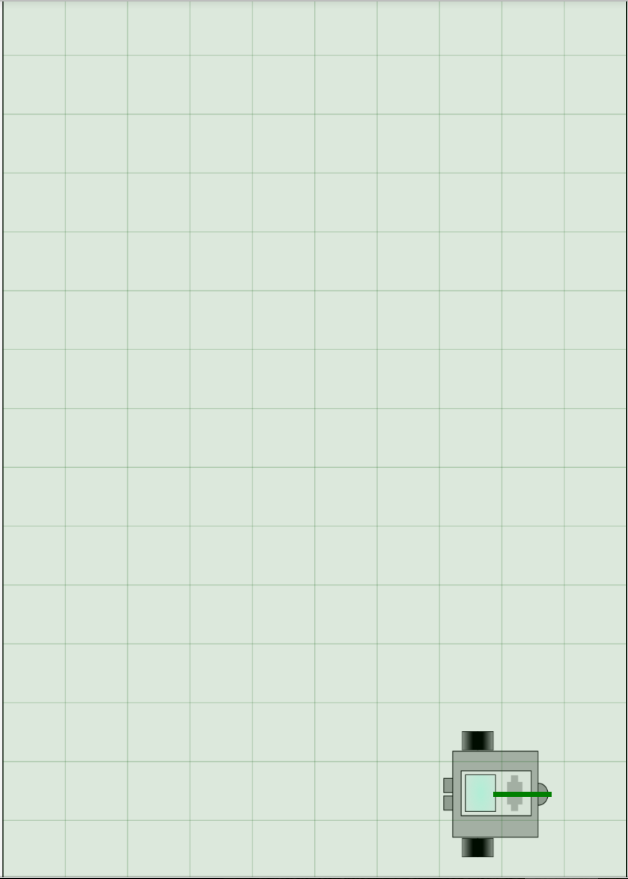
\includegraphics[width=0.95\linewidth]{MapArea.png}  
		\caption{Map Area}
		\label{fig:Map Area}                
	\end{subfigure}
	\begin{subfigure}[t]{0.25\textwidth}
		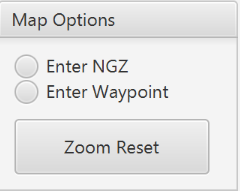
\includegraphics[width=0.95\linewidth]{MapOptions.png}  
		\caption{Map Options}
		\label{fig:Map Options}                
	\end{subfigure}
	\begin{subfigure}[t]{0.25\textwidth}
		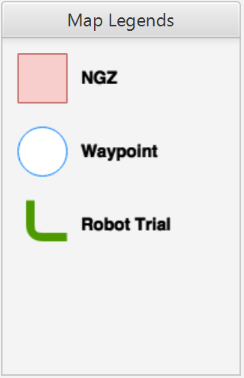
\includegraphics[width=0.95\linewidth]{maplegends.png}  
		\caption{Map Legends}
		\label{fig:Map Legends}                
	\end{subfigure}
	\caption{Map Panel Components}
\end{figure}

\begin{table}[]
	\centering
	\caption{Methods called by map listeners}
	\label{Methods called by map listeners}
	\begin{tabular}{|l|l|}
		\hline
		\textbf{Name}             & Mouse Action and Action                                                                                                                                                                                                                             \\ \hline
		\textbf{onClickZoomReset} & Click on the reset button                                                                                                                                                                                                                           \\ \hline
		\textbf{onClickMap}       & Selecting the mode for map input, Enter NGZ or Enter waypoint \\ \hline
		\textbf{onDragMap}        & Determine the map action, the user do not need to concern this method                                                                                                                                                                               \\ \hline
	\end{tabular}
\end{table}

\textbf{Status and Logging Panels}\\
The user can check the EV3 hardware status such as colour and ultrasonic sensors and switch the robot from manual mode to auto survey mode or menus through the status panel shown as Fig.\ref{fig:panelStatus}. Also, the user can check the system log through the log console shown as Fig.\ref{fig:panelLog}.

\begin{figure}[H]
	\centering
	\begin{subfigure}[t]{0.5\textwidth}
		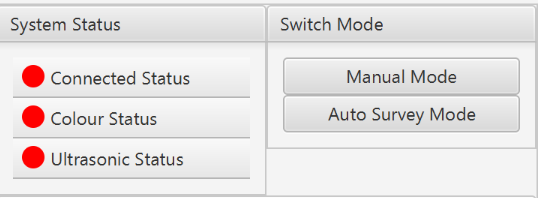
\includegraphics[width=0.95\linewidth]{Systemstatus.png}  
		\caption{System Status}
		\label{fig:panelStatus}                
	\end{subfigure}
	\begin{subfigure}[t]{0.45\textwidth}
		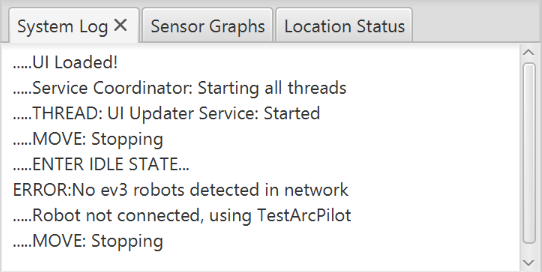
\includegraphics[width=0.95\linewidth]{SystemLog.png}  
		\caption{System Log}
		\label{fig:panelLog}
	\end{subfigure}
	\caption{Status Panels}
\end{figure}

\textbf{Other Functionalities}\\
The User can import and export the map XML file through the File button shown as Fig. \ref{fig:other topmenu}. When the user import the map XML file, the map will show the obstacle, trail or track which are described in the XML file immediately. Also, if user has any operation issue, the use can click help button to find the manual for operating the software(shown as Fig. \ref{fig:other_help}). The user can check the current version of the software through about button(show as Fig.\ref{fig:other_about}).

\begin{figure}[H]
	\centering
	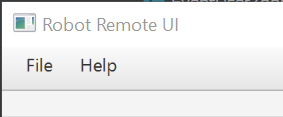
\includegraphics[width=50mm]{other.png}  
	\caption{Other Menu Functions}
	\label{fig:other topmenu}                
\end{figure}

\begin{figure}[H]
	\centering
	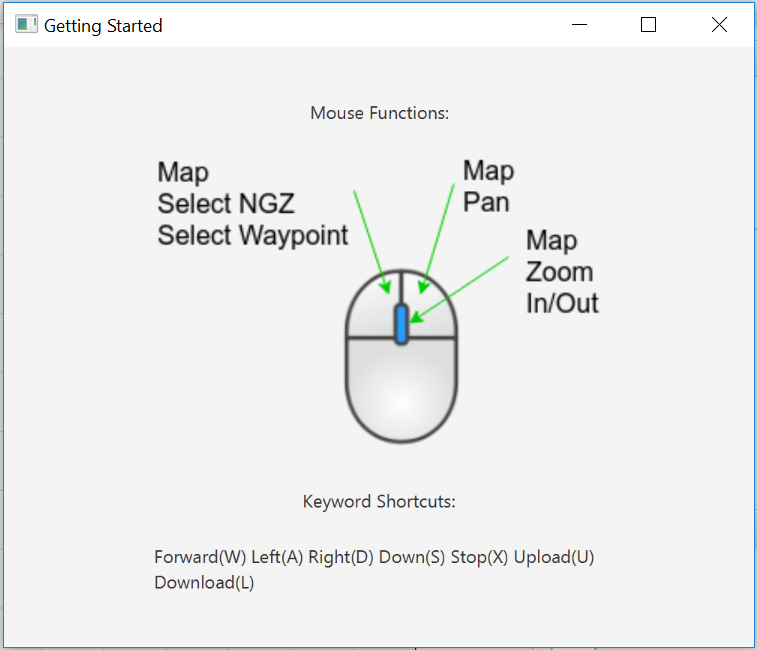
\includegraphics[width=80mm]{Help.png}  
	\caption{Help Popup Window}
	\label{fig:other_help}                
\end{figure}

\begin{figure}[H]
	\centering
	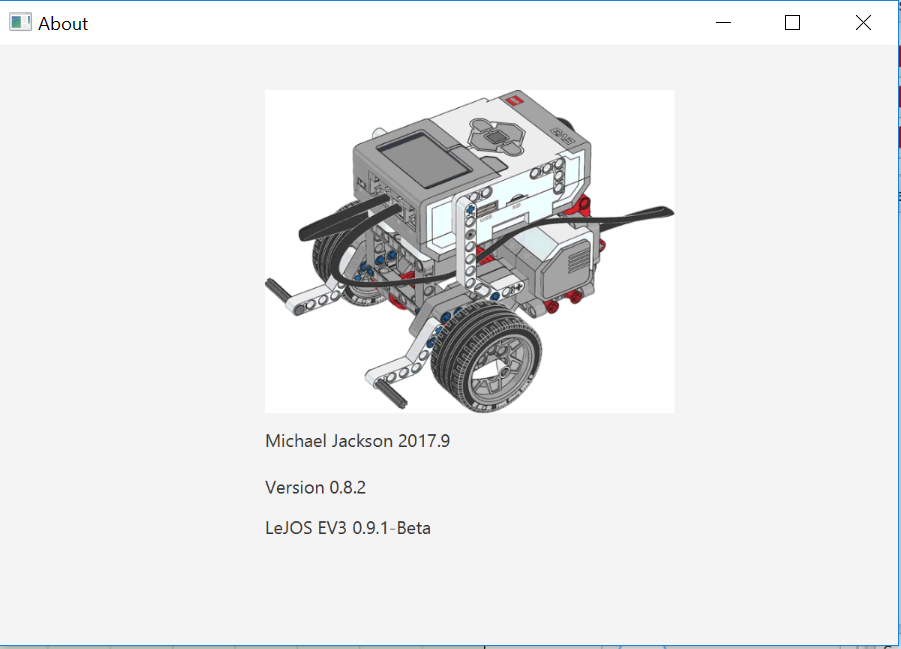
\includegraphics[width=80mm]{About.png}  
	\caption{About Popup Window}
	\label{fig:other_about}
\end{figure}
